\subsection{Relevance to Other Formats}
\label{sec:other-formats}

Many of the terms and general concepts that have driven our PDF work
can be applied to other formats. Potentially any file format that that supports random access or relies on file offsets may have a Trust Chain.

For example, the authors also reviewed the ICC \cite{isotc130jwg7ISO15076120102010} and 
iccMAX \cite{iccSpecificationICC20192019} binary file format that define color profiles.
ICC profiles can be embedded within PDF, JPEG, TIFF and many other formats, but are also 
used independently in operating systems and with embedded devices for managing color in 
printers, displays, cameras, etc.

\begin{figure}[t]
    \centering
    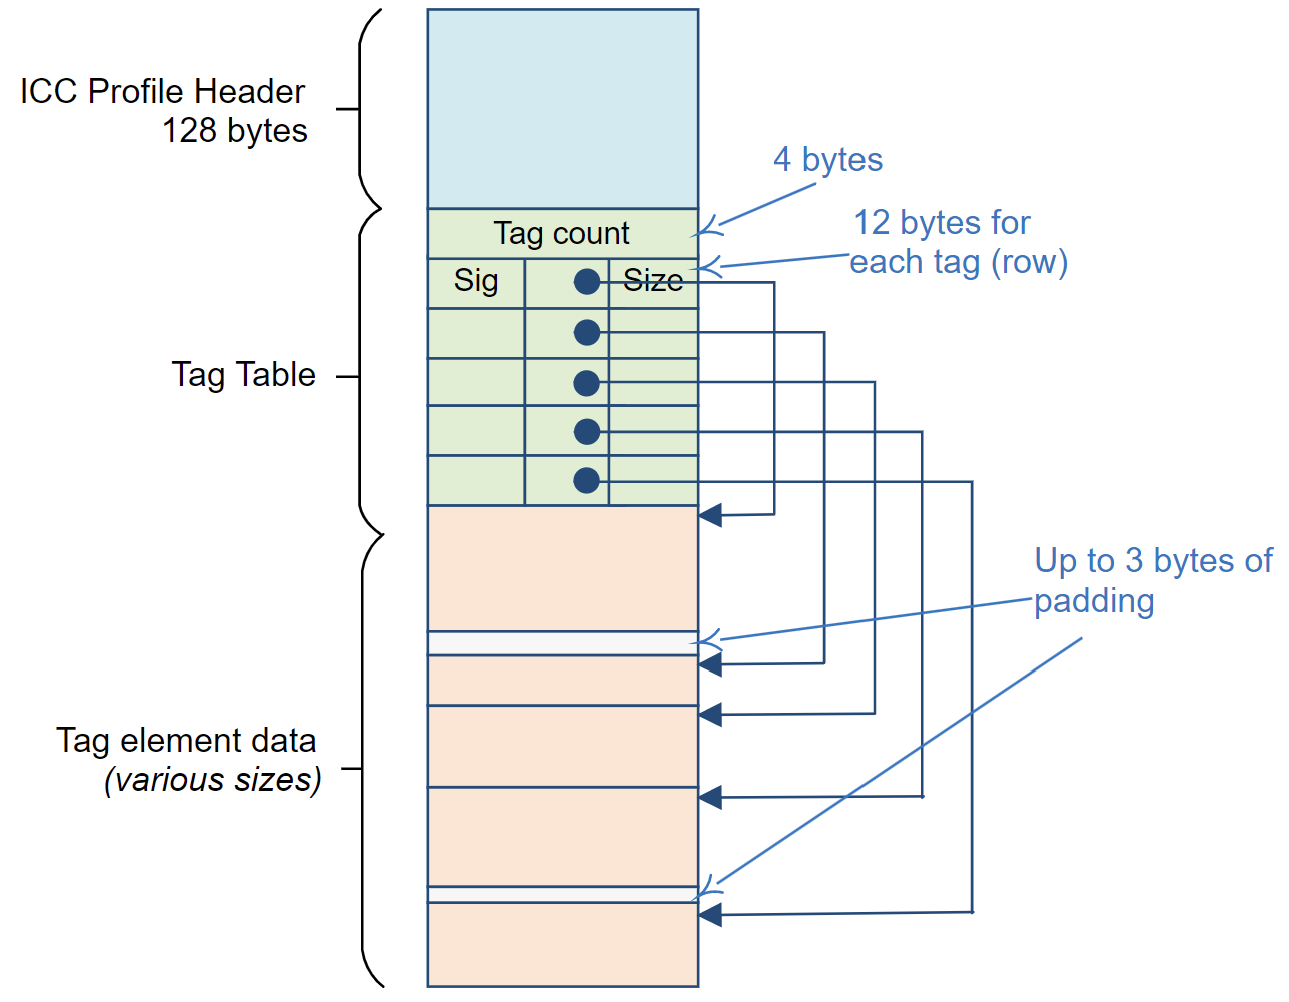
\includegraphics[width=0.85\linewidth]{figures/icc.png}
    \caption{ICC File Structure.}
    \label{fig:icc-structure}
\end{figure}

As shown in \cref{fig:icc-structure} the ICC file structure comprises a 128 byte Header, followed by a 
Tag Table containing byte offsets to various Tag Element Data sections later in the file. 
The Tag Table itself comprises a 4-byte Tag Count followed by tag records, with one record for tag. 
Each record contains 3 4-byte fields: the Tag itself, a file offset to the Tag element data, and the size of the Tag element data (in bytes).
The ICC specifications permit that Tag element data can be reused, so multiple tags in the Tag Table can
refer to the same file location. The ICC specification also requires that tags start on 4-byte boundaries
which means that up to 3 bytes of padding may be required between Tag element data segments.

However when multiple ICC parser implementations were tested, many of these file structure requirements
were not being enforced allowing the authors to create fully functional ICC/PDF polyglots 
without detection.

As a result of our work and that of other researchers in the DARPA-funded ``SafeDocs'' program, several
improvement suggestions have been provided to the ICC.
